\subsection{问题三的模型建立与求解}
\label{sec:q3}
\subsubsection{问题分析与建模思路}
问题三要求在输出情感极性与强度的同时，确定主要参考模态、量化模态作用程度，并定位可回看至原始素材的局部证据。为此，建立输入干预联盟Shapley解释模型（ICF-Shapley），按“情感预测、模态贡献分解、局部证据定位、原素材回映”四个步骤求解。

模型由子集感知预测器（SAP）与两级解释方法组成。预测器采用三态输入和双向时序编码，在附件2上独立训练；模态层精确枚举文本、语音和视觉的8个联盟，以Shapley值分配预测变化；片段层逐块删除输入，以固定类别的预测响应衡量局部作用。沿用前两问的内容掩码、观测掩码及原词时间区间记号，预测器关闭补全分支，使干预后的输入状态由观测掩码直接控制。

\subsubsection{数据准备}
\paragraph{输入组织与可用模态}
采用附件2的对齐版特征，训练、验证、测试样本分别为3395、728、727条，文本、语音和视觉特征形状分别为$50\times768$、$50\times74$和$50\times35$。以$P_{ik}$表示内容掩码，$O^m_{ik}$表示模态$m$的观测掩码；标准化统计量仅由训练集观测位置估计。文本使用冻结的\file{bert-base-uncased}编码，训练与专项推理保持同一接口。

附件4包含20条样本，共564个内容锚点，单条长度介于11与48之间。第13条视觉特征在30个内容位置均为零，因此将该特征分支标记为不可用。定义
\begin{equation}
L_i=\sum_kP_{ik},\quad \mathcal A_i=\{m\in\mathcal M:\sum_kO^m_{ik}>0\},\quad
\rho_i^m=\frac{\sum_kO^m_{ik}}{L_i},\qquad\mathcal M=\{t,a,v\}.
\end{equation}
其中$\rho_i^m$描述观测比例。不可用模态在所有联盟中保持缺失，输出贡献记为NA；该标记描述特征文件的可用性。

\paragraph{片段划分与时间回映}
将内容区划分为不重叠的2锚点块$E$，末块允许不足2个锚点。解释时保持序列长度和位置不变，仅改变相应输入及观测状态。文本块先替换为\file{[UNK]}，再对整句重新编码；语音和视觉块通过观测掩码删除。

附件4原始转写与音轨经词级CTC强制对齐，得到原词区间$A_{iu}=[a_{iu},b_{iu})$。若块$E$对应原词集合$\mathcal U_i(E)=\{g_i(k):k\in E\}$，则证据时间范围为
\begin{equation}
I_i(E)=\left[\min_{u\in\mathcal U_i(E)}a_{iu},\ \max_{u\in\mathcal U_i(E)}b_{iu}\right).
\end{equation}
包含部分子词时按所属原词完整区间回映。逐位核验分词序列后，仅对已获得有效词区间的证据输出秒数，并按真实视频PTS提取距区间中点最近的关键帧；其余保留锚点索引与状态标记。

\subsubsection{模型构建}
\paragraph{三态投影与时序编码}
令$s^m_{ik}\in\{0,1,2\}$分别表示结构填充、已观测和内容缺失。最终采用单层预测器，其输入表示为
\begin{equation}
z^m_{ik}=\operatorname{Lin}_m(X^m_{ik})+e_m^{\mathrm{mod}}+e_k^{\mathrm{pos}}+e^{\mathrm{state}}_{s^m_{ik}},\qquad
\widetilde z^m_{ik}=O^m_{ik}z^m_{ik}+P_{ik}(1-O^m_{ik})e_m^{\mathrm{miss}}.
\end{equation}
按内容长度打包序列，分别输入逐模态双向GRU，避免结构填充参与递归。设隐藏维度为$d$，对各模态内容位的编码结果$h^m_{ik}$分别取均值与最大值，再拼接观测比例：
\begin{equation}
u_i=\operatorname{Concat}_{m\in\mathcal M}\left(\frac1{L_i}\sum_kh^m_{ik},\max_kh^m_{ik}\right)
\mathbin\Vert[\rho_i^t,\rho_i^a,\rho_i^v],\qquad h_i=\operatorname{MLP}(u_i).
\end{equation}
融合向量维度为$6d+3$，分类与回归头分别输出
\begin{equation}
p_i=\operatorname{softmax}(W_ch_i+b_c),\qquad \widehat r_i=3\tanh(W_rh_i+b_r).
\end{equation}

\paragraph{子集训练与目标函数}
最终采用C0方案：以0.70的概率保留全部模态，其余0.30均匀分配给7个非完整联盟，包含空集。对采样联盟$S_i$，令$\widetilde O^m_{ik}=O^m_{ik}\mathbf1\{m\in S_i\}$。训练目标为
\begin{equation}
\mathcal L_3=\operatorname{CE}_w(y_i,p_i)+\operatorname{Huber}_1(r_i,\widehat r_i)
+0.2\left[(p_{i,+}-p_{i,-})-\tanh(\widehat r_i/3)\right]^2.
\end{equation}
类别权重由训练集频数确定，Huber损失拟合连续强度，最后一项约束两类输出的方向一致性。该方案覆盖模态联盟输入；连续片段遮挡增广及更深网络作为候选变体单独比较。

\paragraph{模态贡献与主要参考模态}
以三种子平均概率$\bar p_i$确定原始可用输入的参考类别$c_i^*=\arg\max_c\bar p_{ic}(\mathcal A_i)$，解释全过程固定该类别。对联盟$S\subseteq\mathcal M$，定义
\begin{equation}
F_i^{\mathrm{cls}}(S)=\log\frac{\bar p_{i,c_i^*}(S)}{1-\bar p_{i,c_i^*}(S)},\qquad
F_i^{\mathrm{reg}}(S)=\overline{\widehat r}_i(S).
\end{equation}
数值计算时将概率截断至$[10^{-6},1-10^{-6}]$。对分类与强度分别计算Shapley贡献：
\begin{equation}
\phi_i^m=\sum_{S\subseteq\mathcal M\setminus\{m\}}\frac{|S|!(2-|S|)!}{3!}
\left[F_i(S\cup\{m\})-F_i(S)\right],\qquad
\sum_{m\in\mathcal A_i}\phi_i^m=F_i(\mathcal A_i)-F_i(\varnothing).
\end{equation}
贡献为正表示相对基线抬高价值，为负表示压低价值。以分类贡献绝对值最大的可用模态为主要参考模态，作用份额定义为
\begin{equation}
m_i^*=\arg\max_{m\in\mathcal A_i}|\phi_i^{m,\mathrm{cls}}|,\qquad
\omega_i^m=\frac{|\phi_i^{m,\mathrm{cls}}|}{\sum_{j\in\mathcal A_i}|\phi_i^{j,\mathrm{cls}}|}.
\end{equation}
当总贡献幅度小于$10^{-8}$时标记为无法区分；其余同时报告作用份额与有符号贡献，以区分作用大小和方向。

\paragraph{局部证据与解释评价}
记$F_i^{\mathrm{cls,del}(m,E)}$为仅删除模态$m$中块$E$后的固定类别价值，定义
\begin{equation}
\Delta_i^m(E)=F_i^{\mathrm{cls}}(\mathcal A_i)-F_i^{\mathrm{cls,del}(m,E)}.
\end{equation}
$\Delta_i^m(E)>0$表示该片段支持参考类别，小于零表示抑制参考类别。对全部可用模态计算逐块响应，并在各模态中按响应降序选取局部证据。

在主要参考模态中，按块数的10\%、20\%、30\%向上取整，分别累计删除高分块、低分块和随机块；随机顺序重复3次，并报告实际锚点覆盖率。以三个删除档位的平均概率下降定义AOPC，按样本配对比较高分与随机删除，采用2000次bootstrap估计区间。条件充分性保留其他模态及主要模态的高分块，计算相对原预测的绝对概率偏差。另以训练集同位置均值（B2）和模态内顺序打乱（B3）替代缺失状态基线（B1），比较主模态一致率及贡献排序。

\subsubsection{模型求解与参数设置}
\paragraph{候选比较与模型选择}
以C0为基准，设置三个递进变体：V1调整联盟采样并加入连续块遮挡；V2进一步采用两层BiGRU、逐模态LayerNorm和回归支路；V3增加联盟单调一致性正则。V1与V2各包含多项联合改动，因此比较反映方案组合的影响。V3约束增补模态后的参考类别响应，其单调性不等价于贡献可加性。

选模指标为$J=\mathrm{Macro\mbox{-}F1}-0.1\mathrm{MAE}$。候选须同时满足：$J$不低于C0减0.002；去文本、去语音、去视觉及全缺失四种状态的平均Macro-F1不低于C0减0.002；解释AOPC差不低于C0减0.005。通过者按缺失状态平均Macro-F1排序，并列时比较$J$。训练早停与变体选择使用验证集，最终在附件2测试集评价预测性能，对附件4输出预测与解释。

\begin{table}[htbp]\centering\small
\caption{最终SAP预测器及解释参数}\label{q3:tab:params}
\begin{tabularx}{\linewidth}{p{3.4cm}Y}\toprule
项目 & 设置\\\midrule
网络 & 投影维度64；单层BiGRU，单方向32；融合MLP；Dropout 0.2\\
优化 & AdamW；学习率0.0015；权重衰减$10^{-4}$；余弦调度\\
训练 & 批量256；至多32轮；早停耐心8；梯度范数上限5；种子0、1、2\\
联盟采样 & 全集0.70，其余7个联盟各$0.30/7$；最终模型无块遮挡增广\\
解释 & 8个联盟精确枚举；局部2锚点块；3组随机删除；样本bootstrap 2000次\\
验证子集 & 固定种子20260925随机抽取96条，用于解释诊断和候选比较\\
计算环境 & Python 3.12；PyTorch 2.8.0+cu128；RTX 5060 Ti\\\bottomrule
\end{tabularx}\end{table}

\begin{algorithm}[htbp]
\caption{ICF-Shapley预测与证据定位}\label{q3:alg}\small
\textbf{输入：}三模态特征、掩码、原始素材、冻结预测器与标准化参数。\par
\textbf{输出：}情感极性、强度、模态贡献、主要参考模态及局部证据。\par
\begin{enumerate}
\item 计算可用集合$\mathcal A_i$与集成预测，固定参考类别$c_i^*$。
\item 枚举8个模态联盟，计算分类log-odds与预测强度。
\item 求解两类Shapley值，核验效率性，输出$\omega_i^m$与$m_i^*$。
\item 遍历各可用模态的2锚点块，实施输入删除，计算$\Delta_i^m(E)$。
\item 选择各模态最高分片段，由原词CTC区间及视频PTS定位证据。
\item 保存预测、贡献与逐块响应，生成解释卡；在验证子集评价忠实性、条件充分性及稳定性。
\end{enumerate}
\end{algorithm}

\subsubsection{实验结果与分析}
\paragraph{预测性能与候选比较}
按三项门槛选择的预测器为C0 对照（原训练分布）。三个种子分别在第4、5、3轮取得最优验证指标，训练轮次完全由验证集$J$决定，测试集与附件4只参与前向计算。验证集单种子Macro-F1为0.6068、0.5941、0.6082，三种子集成后为0.6170；测试集Macro-F1为0.6054，MAE为0.6303。
\begin{table}[htbp]\centering\small
\caption{SAP三种子集成的预测性能}\label{q3:tab:perf}
\begin{tabular}{lrrrr}\toprule
数据集 & Accuracy & Macro-F1 & MAE & Pearson\\\midrule
验证集 & 0.6264 & 0.6170 & 0.5954 & 0.6420 \\
测试集 & 0.6286 & 0.6054 & 0.6303 & 0.6730 \\
\bottomrule\end{tabular}\end{table}
验证集负向、中性、正向F1依次为0.6430、0.5114与0.6966，类别间的差异集中在中间类别，中性边界的刻画是提升分类表现的关键环节。图\ref{q3:fig:perf}给出类别间的混淆结构与各类别指标。
\begin{figure}[htbp]\centering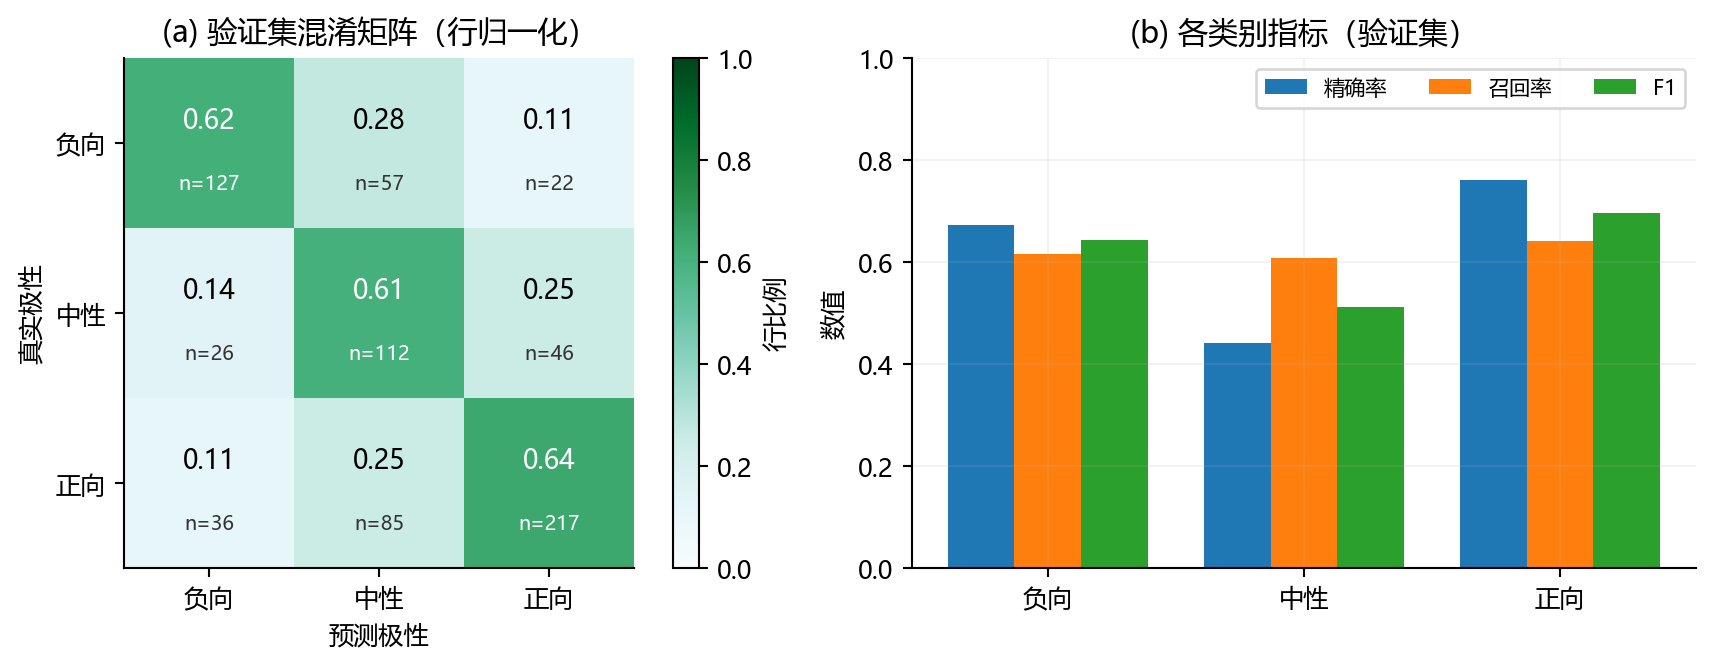
\includegraphics[width=.92\linewidth]{figures/q3_performance.png}
\caption{验证集混淆矩阵与分类指标。}\label{q3:fig:perf}\end{figure}

\begin{table}[htbp]\centering\small
\caption{候选方案与实现对照的验证结果}\label{q3:tab:ablation}
\begin{tabular}{lrrrrr}\toprule
方案 & $J$ & Macro-F1 & MAE & AOPC差 & 种子一致率\\\midrule
仅完整输入（单种子） & 0.5470 & 0.6073 & 0.6030 & --- & --- \\
无内容区打包对照 & 0.5468 & 0.6073 & 0.6048 & --- & --- \\
C0：子集训练 & 0.557 & 0.6170 & 0.5954 & 0.107 & 84.0\% \\
V1：采样与遮挡 & 0.553 & 0.6112 & 0.5869 & 0.130 & 77.8\% \\
V2：增加容量 & 0.553 & 0.6128 & 0.6010 & 0.112 & 79.2\% \\
V3：单调正则 & 0.559 & 0.6192 & 0.6011 & 0.124 & 75.7\% \\
\bottomrule\end{tabular}\end{table}
V1未通过预测指标与缺失状态性能门槛，V2未通过预测指标门槛，V3未通过缺失状态性能门槛；三者的解释AOPC差均达到门槛。据此选择C0作为最终SAP预测器，后续贡献分解和附件4推理均使用该模型。内容区打包与全序列编码的各单种子$J$平均值分别为0.542和0.539。表中仅完整输入对照采用单种子，其余方案采用三种子集成；种子一致率指主要参考模态的两两一致率平均值。
整模态删除给出模态重要性的独立证据：C0去文本后的Macro-F1为0.4150，而去语音、去视觉后分别为0.6092与0.5974，相对完整输入的0.6170，文本删除造成的下降最大，与联盟分解中文本主导的结论一致。仅用完整输入训练的单种子模型去文本后降至0.2904；两者集成规模不同，该差值同时包含训练方案与集成的影响。全缺失条件仅用于输入状态诊断，其预测仍可利用保留的内容长度。

\paragraph{模态作用差异}
空集价值为-0.687，全模态价值为0.542，单模态联盟中文本为0.382、语音为-0.651、视觉为-0.637；三模态平均Shapley贡献为文本+1.105、语音+0.068、视觉+0.056，96条子集中分类主参考模态为文本86条、语音3条、视觉7条。
图\ref{q3:fig:coal}显示，文本的平均Shapley贡献为$+1.105$，构成预测的主导信息来源；语音与视觉分别贡献$+0.068$与$+0.056$，在三模态协同中提供补充信息，主参考模态分布与贡献排序一致。样本层的正负贡献与主参考模态另行保留，以刻画个体差异。效率性残差不超过$8.9\times10^{-16}$，满足Shapley效率性公理。
\begin{figure}[htbp]\centering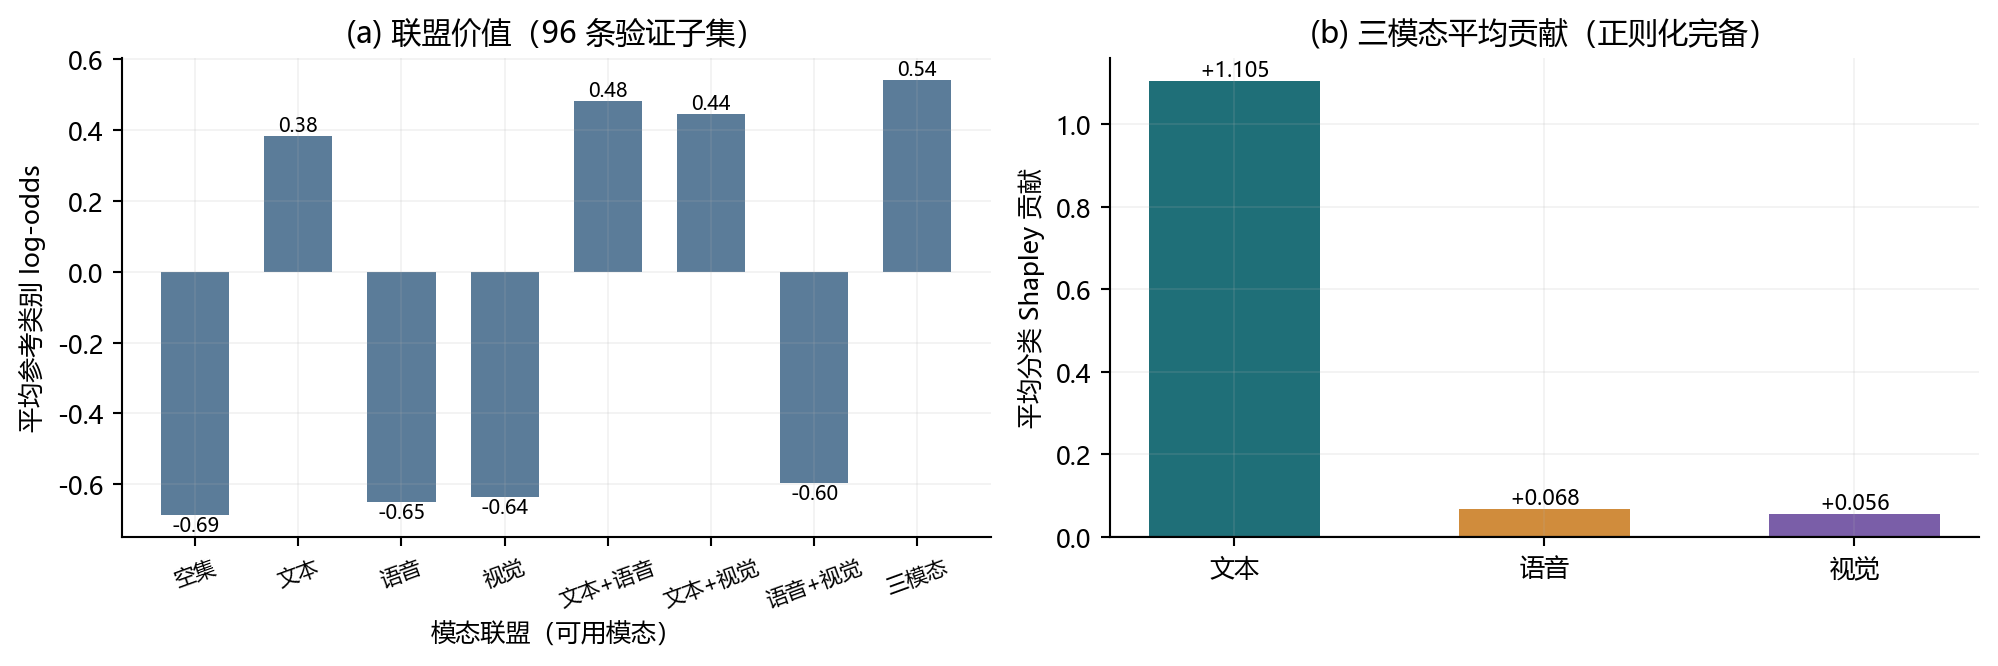
\includegraphics[width=.94\linewidth]{figures/q3_coalition_value.png}
\caption{模态联盟的平均分类价值与三模态平均Shapley贡献。}\label{q3:fig:coal}\end{figure}

\paragraph{局部证据与解释检验}
位置级证据由输入干预直接度量：96条验证样本共完成3397个局部块干预，文本、语音与视觉的平均绝对log-odds响应分别为0.377、0.015与0.025，与模态级贡献的结论一致，均以文本为主。典型样本的逐块分布见图\ref{q3:fig:card1}，累计删除结果见图\ref{q3:fig:faith}。
按块数10\%、20\%、30\%三个目标档位累计删除时，高分块引起的参考类别概率下降分别为0.187、0.226、0.241，随机块为0.075、0.111、0.148，低分块为-0.014、0.006、0.038；高分块与随机块的样本级配对差为0.1068（95\%区间[0.0887,0.1259]），实际覆盖率为14.41\%、24.03\%、35.49\%。条件充分性在最高档的绝对概率偏差为0.1608，表明主要模态中被舍弃的片段对预测仍有贡献。图\ref{q3:fig:faith}(b)给出解释方法的对照结果：B1/B2/B3三种基线下的主模态一致率分别为100.00\%、90.62\%与87.50\%，绝对贡献排序的Spearman相关为0.812与0.625，主要参考模态的判定不依赖具体基线。同一删除协议在强度回归头上给出相同的排序：删除高分块10\%、20\%、30\%时强度的绝对变化为0.399、0.468与0.499，删除低分块为0.142、0.192与0.227，两组差距随删除比例扩大，局部证据排序对连续强度输出同样成立。在主参考模态为文本的86条样本中，最高分证据块完全由功能词或标点构成的比例为17.4\%，低于全部文本块基线的30.5\%，配对差为-0.130（95\%区间[-0.212,-0.046]），最高分证据落点集中在实词上。
\begin{figure}[htbp]\centering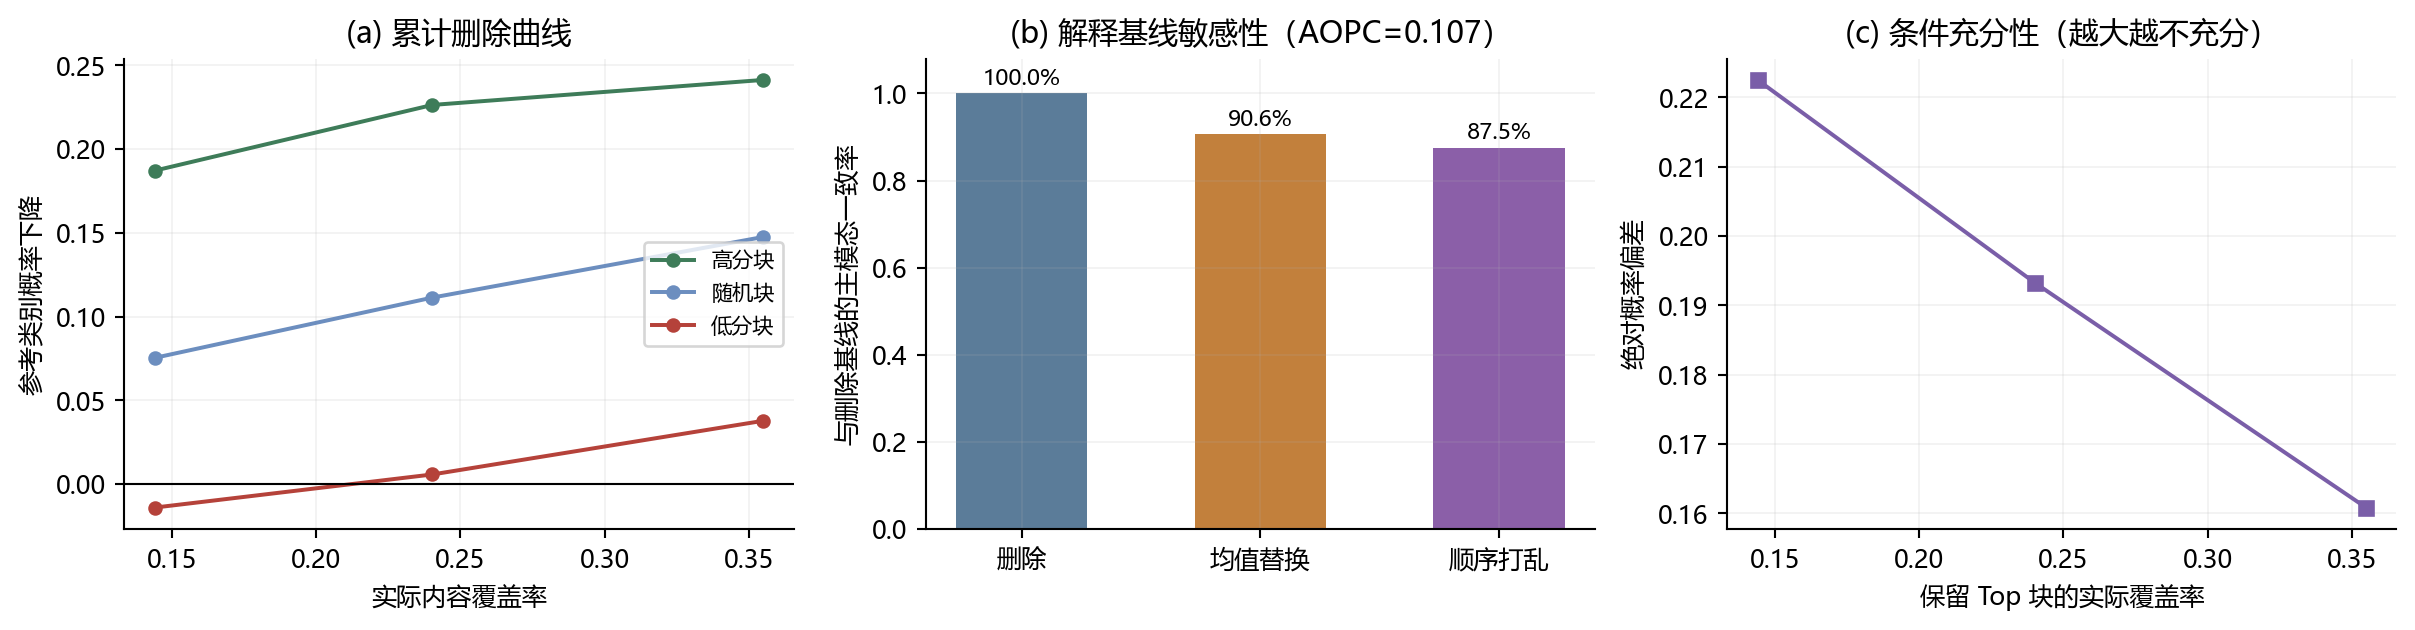
\includegraphics[width=\linewidth]{figures/q3_faithfulness.png}
\caption{高分、随机与低分块累计删除对比、基线敏感性及条件充分性。}\label{q3:fig:faith}\end{figure}
训练随机性与解释基线分别检验解释的稳定性：三种子两两的主参考模态一致率为82.29\%、83.33\%与86.46\%，B1/B2/B3三种基线下的主模态一致率分别为100.00\%、90.62\%与87.50\%。输入删除能够稳定识别对当前预测作用较强的片段；上述96条样本同时参与候选比较，置信区间描述该验证子集上的配对差异。

\paragraph{错误分布与归因分析}
验证集共272条误判，其中214条涉及中性，占78.7\%。按真实分组看：中性组错误率39.1\%（184条），非中性且|强度|<0.5的弱情感组错误率60.5\%（147条），|强度|≥0.5的强情感组错误率28.0\%（397条）。错误随情感强度降低而集中，说明零点附近的类别判别比强情感的方向判断更困难。

在96条解释样本中，低强度组与高强度组的解释不稳定率分别为31.7\%和23.6\%，覆盖正确与错误预测两类样本，给出解释稳定性在不同强度水平上的分布。错误分析将改进重点指向中性边界与弱情感区间的表征增强。

\paragraph{附件4全量结果}
附件4全部20条样本的预测分布为中性7条、负向7条、正向6条，分类主参考模态为文本19条、视觉1条。图\ref{q3:fig:a4}给出全量预测、模态份额和种子间波动，表\ref{q3:tab:all20}列出逐条数值。20条样本的强度三种子标准差均值为0.105，最大为0.410（附件4\_10）。第13条的视觉分支不可用，其视觉份额标记为NA，其余两个模态照常给出贡献；4-04与4-19的预测极性与强度方向不一致，属于独立双头结构下的输出分歧，两个任务分别保留各自的预测与贡献分解。
\begin{figure}[htbp]\centering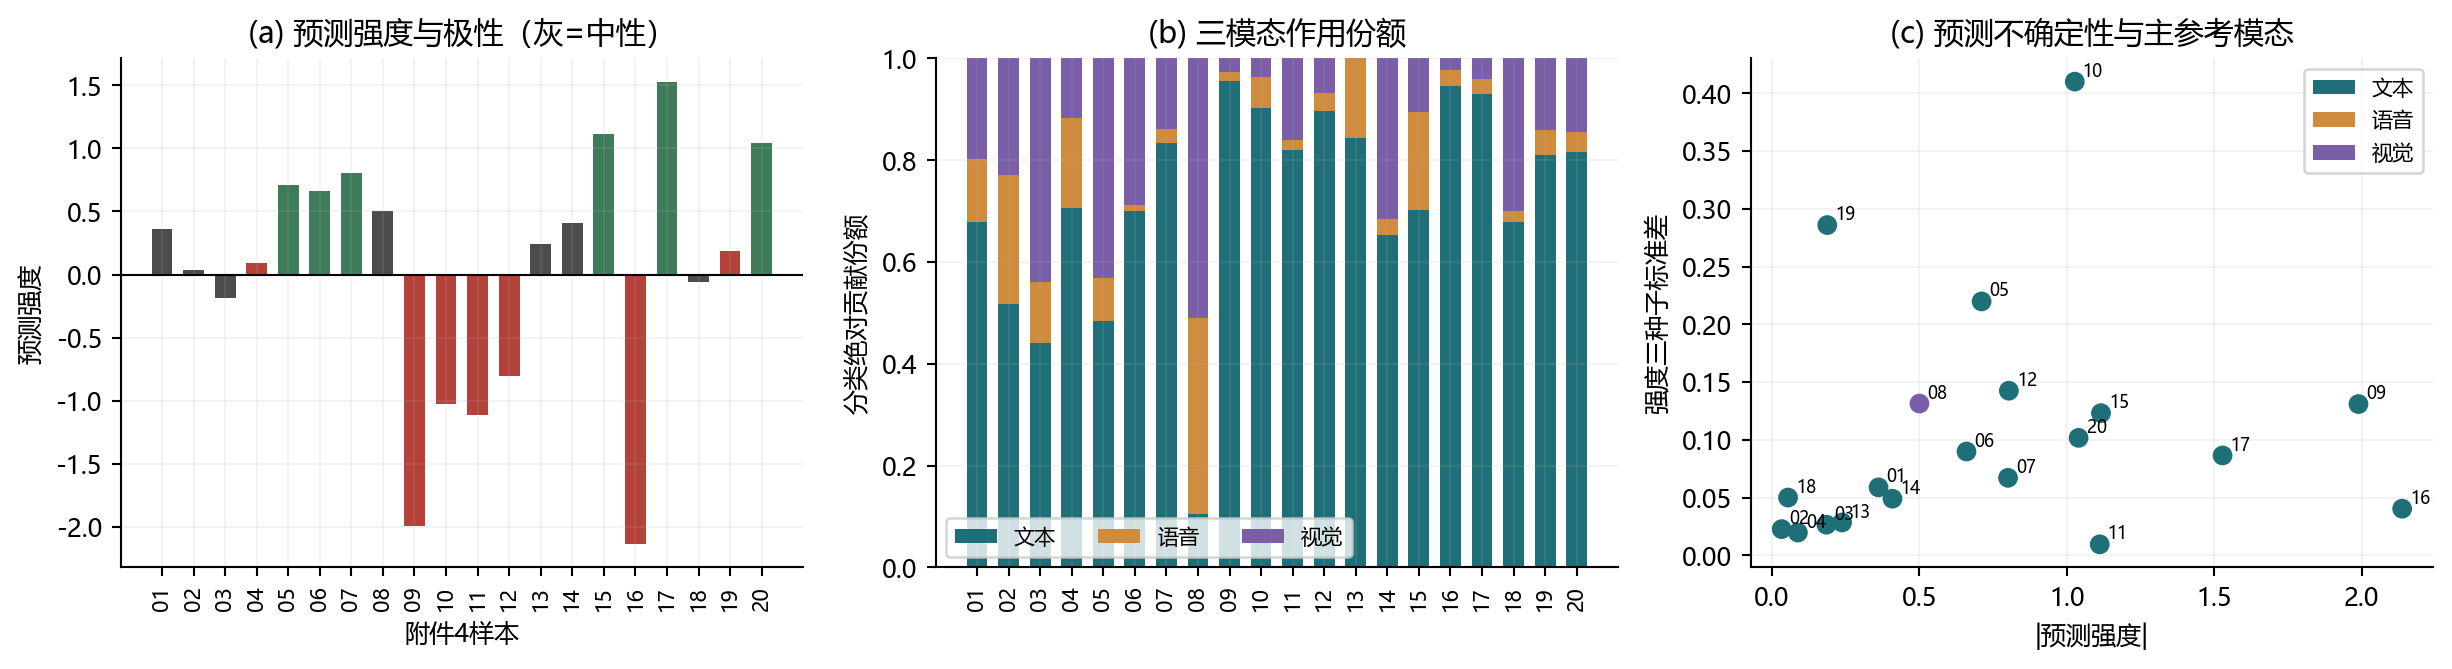
\includegraphics[width=\linewidth]{figures/q3_a4_overview.png}
\caption{附件4全部20条样本的情感预测、模态作用份额与种子间波动。}\label{q3:fig:a4}\end{figure}
\begin{table}[htbp]\centering\small
\caption{附件4全量预测与分类模态作用份额}\label{q3:tab:all20}
\begin{tabular}{clrrrrl}\toprule
编号 & 极性 & 强度 & 文本份额 & 语音份额 & 视觉份额 & 主模态\\\midrule
4-01 & 中性 & +0.362 & 0.678 & 0.124 & 0.198 & 文本 \\
4-02 & 中性 & +0.034 & 0.518 & 0.254 & 0.229 & 文本 \\
4-03 & 中性 & -0.185 & 0.441 & 0.119 & 0.440 & 文本 \\
4-04 & 负向 & +0.089 & 0.705 & 0.178 & 0.116 & 文本 \\
4-05 & 正向 & +0.711 & 0.484 & 0.085 & 0.432 & 文本 \\
4-06 & 正向 & +0.660 & 0.699 & 0.014 & 0.287 & 文本 \\
4-07 & 正向 & +0.801 & 0.833 & 0.029 & 0.138 & 文本 \\
4-08 & 中性 & +0.501 & 0.106 & 0.384 & 0.510 & 视觉 \\
4-09 & 负向 & -1.989 & 0.955 & 0.018 & 0.027 & 文本 \\
4-10 & 负向 & -1.027 & 0.903 & 0.060 & 0.037 & 文本 \\
4-11 & 负向 & -1.112 & 0.820 & 0.020 & 0.160 & 文本 \\
4-12 & 负向 & -0.804 & 0.897 & 0.036 & 0.067 & 文本 \\
4-13 & 中性 & +0.238 & 0.844 & 0.156 & NA & 文本 \\
4-14 & 中性 & +0.409 & 0.654 & 0.031 & 0.315 & 文本 \\
4-15 & 正向 & +1.116 & 0.703 & 0.192 & 0.105 & 文本 \\
4-16 & 负向 & -2.137 & 0.946 & 0.031 & 0.022 & 文本 \\
4-17 & 正向 & +1.528 & 0.930 & 0.029 & 0.040 & 文本 \\
4-18 & 中性 & -0.055 & 0.679 & 0.021 & 0.300 & 文本 \\
4-19 & 负向 & +0.188 & 0.809 & 0.049 & 0.141 & 文本 \\
4-20 & 正向 & +1.040 & 0.816 & 0.040 & 0.144 & 文本 \\
\bottomrule\end{tabular}\end{table}
\file{pred\_附件4.csv}保存预测及分类、强度的有符号贡献；\file{explain\_附件4.csv}按样本和模态保存证据片段、时间与媒体索引，共60行，包含不可用状态；\file{local\_blocks\_附件4.csv}保存全部逐块响应。

\paragraph{典型样本与证据回映}
选取附件4第1条展示完整解释链条。第1条预测为中性，强度+0.362，主要参考模态为文本（份额0.678），最高分证据片段为\textit{the timing}，估计时间2.62--3.00\,s。 图\ref{q3:fig:card1}同时展示预测结果、三模态作用程度、主要模态的逐块响应与原始关键帧；响应的正负分别对应支持和抑制作用。
\begin{figure}[htbp]\centering\includegraphics[width=.90\linewidth]{figures/q3_card_01.png}
\caption{附件4第1条解释卡：预测、模态份额、局部片段重要性与关键证据定位。}\label{q3:fig:card1}\end{figure}
回映覆盖情况如下：20条样本的重新分词序列均与官方词元一致，482个原词中478个获得CTC时间区间；59条可用模态证据中58条完成时间回映，时间区间由CTC词级对齐给出，未获得词区间的证据以锚点索引记录。第13条的视觉特征不可用，其解释保留文本与语音贡献，并在全量文件中标记为视觉NA。

本模型把情感预测分解为可复核的模态贡献与局部响应，并通过词级时间区间连接到原始素材：Shapley值度量指定模型与基线下的作用差异，删除实验检验局部证据与预测响应的一致性。两项分析在同一预测器上完成，因此解释结论可直接对应该模型的决策过程。
\FloatBarrier
